\documentclass[twoside]{book}

% Packages required by doxygen
\usepackage{fixltx2e}
\usepackage{calc}
\usepackage{doxygen}
\usepackage[export]{adjustbox} % also loads graphicx
\usepackage{graphicx}
\usepackage[utf8]{inputenc}
\usepackage{makeidx}
\usepackage{multicol}
\usepackage{multirow}
\PassOptionsToPackage{warn}{textcomp}
\usepackage{textcomp}
\usepackage[nointegrals]{wasysym}
\usepackage[table]{xcolor}

% Font selection
\usepackage[T1]{fontenc}
\usepackage[scaled=.90]{helvet}
\usepackage{courier}
\usepackage{amssymb}
\usepackage{sectsty}
\renewcommand{\familydefault}{\sfdefault}
\allsectionsfont{%
  \fontseries{bc}\selectfont%
  \color{darkgray}%
}
\renewcommand{\DoxyLabelFont}{%
  \fontseries{bc}\selectfont%
  \color{darkgray}%
}
\newcommand{\+}{\discretionary{\mbox{\scriptsize$\hookleftarrow$}}{}{}}

% Page & text layout
\usepackage{geometry}
\geometry{%
  a4paper,%
  top=2.5cm,%
  bottom=2.5cm,%
  left=2.5cm,%
  right=2.5cm%
}
\tolerance=750
\hfuzz=15pt
\hbadness=750
\setlength{\emergencystretch}{15pt}
\setlength{\parindent}{0cm}
\setlength{\parskip}{3ex plus 2ex minus 2ex}
\makeatletter
\renewcommand{\paragraph}{%
  \@startsection{paragraph}{4}{0ex}{-1.0ex}{1.0ex}{%
    \normalfont\normalsize\bfseries\SS@parafont%
  }%
}
\renewcommand{\subparagraph}{%
  \@startsection{subparagraph}{5}{0ex}{-1.0ex}{1.0ex}{%
    \normalfont\normalsize\bfseries\SS@subparafont%
  }%
}
\makeatother

% Headers & footers
\usepackage{fancyhdr}
\pagestyle{fancyplain}
\fancyhead[LE]{\fancyplain{}{\bfseries\thepage}}
\fancyhead[CE]{\fancyplain{}{}}
\fancyhead[RE]{\fancyplain{}{\bfseries\leftmark}}
\fancyhead[LO]{\fancyplain{}{\bfseries\rightmark}}
\fancyhead[CO]{\fancyplain{}{}}
\fancyhead[RO]{\fancyplain{}{\bfseries\thepage}}
\fancyfoot[LE]{\fancyplain{}{}}
\fancyfoot[CE]{\fancyplain{}{}}
\fancyfoot[RE]{\fancyplain{}{\bfseries\scriptsize Generated by Doxygen }}
\fancyfoot[LO]{\fancyplain{}{\bfseries\scriptsize Generated by Doxygen }}
\fancyfoot[CO]{\fancyplain{}{}}
\fancyfoot[RO]{\fancyplain{}{}}
\renewcommand{\footrulewidth}{0.4pt}
\renewcommand{\chaptermark}[1]{%
  \markboth{#1}{}%
}
\renewcommand{\sectionmark}[1]{%
  \markright{\thesection\ #1}%
}

% Indices & bibliography
\usepackage{natbib}
\usepackage[titles]{tocloft}
\setcounter{tocdepth}{3}
\setcounter{secnumdepth}{5}
\makeindex

% Hyperlinks (required, but should be loaded last)
\usepackage{ifpdf}
\ifpdf
  \usepackage[pdftex,pagebackref=true]{hyperref}
\else
  \usepackage[ps2pdf,pagebackref=true]{hyperref}
\fi
\hypersetup{%
  colorlinks=true,%
  linkcolor=blue,%
  citecolor=blue,%
  unicode%
}

% Custom commands
\newcommand{\clearemptydoublepage}{%
  \newpage{\pagestyle{empty}\cleardoublepage}%
}

\usepackage{caption}
\captionsetup{labelsep=space,justification=centering,font={bf},singlelinecheck=off,skip=4pt,position=top}

%===== C O N T E N T S =====

\begin{document}

% Titlepage & ToC
\hypersetup{pageanchor=false,
             bookmarksnumbered=true,
             pdfencoding=unicode
            }
\pagenumbering{alph}
\begin{titlepage}
\vspace*{7cm}
\begin{center}%
{\Large Password\+Vault }\\
\vspace*{1cm}
{\large Generated by Doxygen 1.8.13}\\
\end{center}
\end{titlepage}
\clearemptydoublepage
\pagenumbering{roman}
\tableofcontents
\clearemptydoublepage
\pagenumbering{arabic}
\hypersetup{pageanchor=true}

%--- Begin generated contents ---
\chapter{Class Index}
\section{Class List}
Here are the classes, structs, unions and interfaces with brief descriptions\+:\begin{DoxyCompactList}
\item\contentsline{section}{\hyperlink{structHeap}{Heap} }{\pageref{structHeap}}{}
\item\contentsline{section}{\hyperlink{structNode}{Node} }{\pageref{structNode}}{}
\end{DoxyCompactList}

\chapter{File Index}
\section{File List}
Here is a list of all documented files with brief descriptions\+:\begin{DoxyCompactList}
\item\contentsline{section}{include/\hyperlink{car_8h}{car.\+h} \\*File containing the function definitions needed for car struct }{\pageref{car_8h}}{}
\end{DoxyCompactList}

\chapter{Class Documentation}
\hypertarget{structuser__struct}{}\section{user\+\_\+struct Struct Reference}
\label{structuser__struct}\index{user\+\_\+struct@{user\+\_\+struct}}


{\ttfamily \#include $<$Password\+Vault.\+h$>$}

\subsection*{Public Attributes}
\begin{DoxyCompactItemize}
\item 
\mbox{\Hypertarget{structuser__struct_aa74330bd94dc3926e50fe022f1c147b7}\label{structuser__struct_aa74330bd94dc3926e50fe022f1c147b7}} 
char {\bfseries username} \mbox{[}100\mbox{]}
\item 
\mbox{\Hypertarget{structuser__struct_abbe8ba686390f2b2cb5be3263f5e1eb5}\label{structuser__struct_abbe8ba686390f2b2cb5be3263f5e1eb5}} 
char {\bfseries password} \mbox{[}100\mbox{]}
\end{DoxyCompactItemize}


\subsection{Detailed Description}
User. It contains elements which is the username or password. 

The documentation for this struct was generated from the following file\+:\begin{DoxyCompactItemize}
\item 
include/\hyperlink{PasswordVault_8h}{Password\+Vault.\+h}\end{DoxyCompactItemize}

\chapter{File Documentation}
\hypertarget{PasswordVault_8h}{}\section{include/\+Password\+Vault.h File Reference}
\label{PasswordVault_8h}\index{include/\+Password\+Vault.\+h@{include/\+Password\+Vault.\+h}}


File containing the function definitions needed for password struct.  


{\ttfamily \#include $<$stdio.\+h$>$}\newline
{\ttfamily \#include $<$stdlib.\+h$>$}\newline
{\ttfamily \#include \char`\"{}Hash\+Table\+A\+P\+I.\+h\char`\"{}}\newline
Include dependency graph for Password\+Vault.\+h\+:
\nopagebreak
\begin{figure}[H]
\begin{center}
\leavevmode
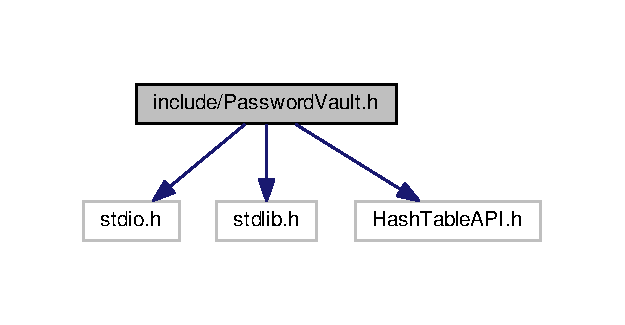
\includegraphics[width=300pt]{PasswordVault_8h__incl}
\end{center}
\end{figure}
\subsection*{Classes}
\begin{DoxyCompactItemize}
\item 
struct \hyperlink{structuser__struct}{user\+\_\+struct}
\end{DoxyCompactItemize}
\subsection*{Typedefs}
\begin{DoxyCompactItemize}
\item 
typedef struct \hyperlink{structuser__struct}{user\+\_\+struct} \hyperlink{PasswordVault_8h_ab1b867c24663b7f952c5897adbd551ac}{User}
\end{DoxyCompactItemize}
\subsection*{Functions}
\begin{DoxyCompactItemize}
\item 
\hyperlink{PasswordVault_8h_ab1b867c24663b7f952c5897adbd551ac}{User} \hyperlink{PasswordVault_8h_af53483090d718ea4cd9529426a26c93c}{create\+User} (H\+Table $\ast$pass\+Vault)
\item 
void \hyperlink{PasswordVault_8h_a3f221ffae84e5a3405fb54ce8641bf92}{signin} (\hyperlink{PasswordVault_8h_ab1b867c24663b7f952c5897adbd551ac}{User} the\+User, H\+Table $\ast$pass\+Vault)
\item 
void \hyperlink{PasswordVault_8h_a630881d89848a65458cbcddbcf448e3b}{add\+Password} (\hyperlink{PasswordVault_8h_ab1b867c24663b7f952c5897adbd551ac}{User} $\ast$the\+User, H\+Table $\ast$pass\+Vault)
\item 
void \hyperlink{PasswordVault_8h_aa48cb4e6a8cd768cab9642a241ec6d41}{change\+Password} (\hyperlink{PasswordVault_8h_ab1b867c24663b7f952c5897adbd551ac}{User} $\ast$the\+User, H\+Table $\ast$pass\+Vault)
\item 
char $\ast$ \hyperlink{PasswordVault_8h_acad2d369f267b9bfb8d1f6cff9244d94}{get\+Password} (\hyperlink{PasswordVault_8h_ab1b867c24663b7f952c5897adbd551ac}{User} $\ast$the\+User, H\+Table $\ast$pass\+Vault)
\item 
void \hyperlink{PasswordVault_8h_a803d2caf86c63568665e06595e73a742}{remove\+Password} (\hyperlink{PasswordVault_8h_ab1b867c24663b7f952c5897adbd551ac}{User} $\ast$the\+User, H\+Table $\ast$pass\+Vault)
\item 
void \hyperlink{PasswordVault_8h_ae6237a49e0d58cca25f0ba5ac3db186f}{load\+File} (\hyperlink{PasswordVault_8h_ab1b867c24663b7f952c5897adbd551ac}{User} the\+User, H\+Table $\ast$pass\+Vault)
\item 
void \hyperlink{PasswordVault_8h_ab1e32487b85d4cec8636606a4f9b003f}{load\+Table} (\hyperlink{PasswordVault_8h_ab1b867c24663b7f952c5897adbd551ac}{User} the\+User, H\+Table $\ast$pass\+Vault)
\item 
void \hyperlink{PasswordVault_8h_a88301cd3c1fe2343a585b34be3400cc3}{print\+Vault} (\hyperlink{PasswordVault_8h_ab1b867c24663b7f952c5897adbd551ac}{User} the\+User, H\+Table $\ast$pass\+Vault)
\item 
H\+Table $\ast$ \hyperlink{PasswordVault_8h_a8182d79e68c3b6536ee84114bb86891b}{create\+Vault} (size\+\_\+t size, int($\ast$\hyperlink{PasswordVault_8h_a0312071e2a498b58a24e35b97ce092de}{hash\+Function})(size\+\_\+t table\+Size, char key\mbox{[}$\,$\mbox{]}), void($\ast$destroy\+Data)(void $\ast$data), void($\ast$print\+Data)(void $\ast$to\+Be\+Printed))
\item 
char $\ast$ \hyperlink{PasswordVault_8h_a1fab5ff4b48141332d9187b51a6dc103}{create\+Pathname} (\hyperlink{PasswordVault_8h_ab1b867c24663b7f952c5897adbd551ac}{User} the\+User)
\item 
int \hyperlink{PasswordVault_8h_a0312071e2a498b58a24e35b97ce092de}{hash\+Function} (size\+\_\+t table\+Size, char key\mbox{[}$\,$\mbox{]})
\item 
void \hyperlink{PasswordVault_8h_a8b61dd28d3f9c9a6806960a8180bee4a}{print\+Password} (void $\ast$to\+Be\+Printed)
\item 
void \hyperlink{PasswordVault_8h_ab5c56aa8ac26781ffd035eae6d942c94}{delete\+Password} (void $\ast$to\+Be\+Deleted)
\item 
int \hyperlink{PasswordVault_8h_a1cbc282300e26607a98ec7c0693687a9}{check\+System} (\hyperlink{PasswordVault_8h_ab1b867c24663b7f952c5897adbd551ac}{User} $\ast$the\+User, H\+Table $\ast$pass\+Vault)
\end{DoxyCompactItemize}


\subsection{Detailed Description}
File containing the function definitions needed for password struct. 

\begin{DoxyAuthor}{Author}
Ralph Arvin De Castro 
\end{DoxyAuthor}
\begin{DoxyDate}{Date}
June 2018 
\end{DoxyDate}


\subsection{Typedef Documentation}
\mbox{\Hypertarget{PasswordVault_8h_ab1b867c24663b7f952c5897adbd551ac}\label{PasswordVault_8h_ab1b867c24663b7f952c5897adbd551ac}} 
\index{Password\+Vault.\+h@{Password\+Vault.\+h}!User@{User}}
\index{User@{User}!Password\+Vault.\+h@{Password\+Vault.\+h}}
\subsubsection{\texorpdfstring{User}{User}}
{\footnotesize\ttfamily typedef struct \hyperlink{structuser__struct}{user\+\_\+struct}  \hyperlink{PasswordVault_8h_ab1b867c24663b7f952c5897adbd551ac}{User}}

User. It contains elements which is the username or password. 

\subsection{Function Documentation}
\mbox{\Hypertarget{PasswordVault_8h_a630881d89848a65458cbcddbcf448e3b}\label{PasswordVault_8h_a630881d89848a65458cbcddbcf448e3b}} 
\index{Password\+Vault.\+h@{Password\+Vault.\+h}!add\+Password@{add\+Password}}
\index{add\+Password@{add\+Password}!Password\+Vault.\+h@{Password\+Vault.\+h}}
\subsubsection{\texorpdfstring{add\+Password()}{addPassword()}}
{\footnotesize\ttfamily void add\+Password (\begin{DoxyParamCaption}\item[{\hyperlink{PasswordVault_8h_ab1b867c24663b7f952c5897adbd551ac}{User} $\ast$}]{the\+User,  }\item[{H\+Table $\ast$}]{pass\+Vault }\end{DoxyParamCaption})}

Function to add password to hashtable 
\begin{DoxyParams}{Parameters}
{\em the\+User} & pointer to user struct with username and password \\
\hline
{\em pass\+Vault} & hashtable that acts as the password vault \\
\hline
\end{DoxyParams}
\mbox{\Hypertarget{PasswordVault_8h_aa48cb4e6a8cd768cab9642a241ec6d41}\label{PasswordVault_8h_aa48cb4e6a8cd768cab9642a241ec6d41}} 
\index{Password\+Vault.\+h@{Password\+Vault.\+h}!change\+Password@{change\+Password}}
\index{change\+Password@{change\+Password}!Password\+Vault.\+h@{Password\+Vault.\+h}}
\subsubsection{\texorpdfstring{change\+Password()}{changePassword()}}
{\footnotesize\ttfamily void change\+Password (\begin{DoxyParamCaption}\item[{\hyperlink{PasswordVault_8h_ab1b867c24663b7f952c5897adbd551ac}{User} $\ast$}]{the\+User,  }\item[{H\+Table $\ast$}]{pass\+Vault }\end{DoxyParamCaption})}

Function to change a password of a system in the hashtable 
\begin{DoxyParams}{Parameters}
{\em the\+User} & pointer to user struct with username and password \\
\hline
{\em pass\+Vault} & hashtable that acts as the password vault \\
\hline
\end{DoxyParams}
\mbox{\Hypertarget{PasswordVault_8h_a1cbc282300e26607a98ec7c0693687a9}\label{PasswordVault_8h_a1cbc282300e26607a98ec7c0693687a9}} 
\index{Password\+Vault.\+h@{Password\+Vault.\+h}!check\+System@{check\+System}}
\index{check\+System@{check\+System}!Password\+Vault.\+h@{Password\+Vault.\+h}}
\subsubsection{\texorpdfstring{check\+System()}{checkSystem()}}
{\footnotesize\ttfamily int check\+System (\begin{DoxyParamCaption}\item[{\hyperlink{PasswordVault_8h_ab1b867c24663b7f952c5897adbd551ac}{User} $\ast$}]{the\+User,  }\item[{H\+Table $\ast$}]{pass\+Vault }\end{DoxyParamCaption})}

Function to check if system exist on hashtable \begin{DoxyReturn}{Returns}
integer that includes the index 
\end{DoxyReturn}

\begin{DoxyParams}{Parameters}
{\em table\+Size} & size of hashtable \\
\hline
{\em key} & character string for password \\
\hline
\end{DoxyParams}
\mbox{\Hypertarget{PasswordVault_8h_a1fab5ff4b48141332d9187b51a6dc103}\label{PasswordVault_8h_a1fab5ff4b48141332d9187b51a6dc103}} 
\index{Password\+Vault.\+h@{Password\+Vault.\+h}!create\+Pathname@{create\+Pathname}}
\index{create\+Pathname@{create\+Pathname}!Password\+Vault.\+h@{Password\+Vault.\+h}}
\subsubsection{\texorpdfstring{create\+Pathname()}{createPathname()}}
{\footnotesize\ttfamily char$\ast$ create\+Pathname (\begin{DoxyParamCaption}\item[{\hyperlink{PasswordVault_8h_ab1b867c24663b7f952c5897adbd551ac}{User}}]{the\+User }\end{DoxyParamCaption})}

Function to create a path name for creating a file \begin{DoxyReturn}{Returns}
character string that contains the pathway 
\end{DoxyReturn}

\begin{DoxyParams}{Parameters}
{\em the\+User} & the user with username and password \\
\hline
\end{DoxyParams}
\mbox{\Hypertarget{PasswordVault_8h_af53483090d718ea4cd9529426a26c93c}\label{PasswordVault_8h_af53483090d718ea4cd9529426a26c93c}} 
\index{Password\+Vault.\+h@{Password\+Vault.\+h}!create\+User@{create\+User}}
\index{create\+User@{create\+User}!Password\+Vault.\+h@{Password\+Vault.\+h}}
\subsubsection{\texorpdfstring{create\+User()}{createUser()}}
{\footnotesize\ttfamily \hyperlink{PasswordVault_8h_ab1b867c24663b7f952c5897adbd551ac}{User} create\+User (\begin{DoxyParamCaption}\item[{H\+Table $\ast$}]{pass\+Vault }\end{DoxyParamCaption})}

Function to create user by creating a bin file as the password vault \begin{DoxyReturn}{Returns}
user struct 
\end{DoxyReturn}

\begin{DoxyParams}{Parameters}
{\em pass\+Vault} & hashtable that includes the usernames and password \\
\hline
\end{DoxyParams}
\mbox{\Hypertarget{PasswordVault_8h_a8182d79e68c3b6536ee84114bb86891b}\label{PasswordVault_8h_a8182d79e68c3b6536ee84114bb86891b}} 
\index{Password\+Vault.\+h@{Password\+Vault.\+h}!create\+Vault@{create\+Vault}}
\index{create\+Vault@{create\+Vault}!Password\+Vault.\+h@{Password\+Vault.\+h}}
\subsubsection{\texorpdfstring{create\+Vault()}{createVault()}}
{\footnotesize\ttfamily H\+Table$\ast$ create\+Vault (\begin{DoxyParamCaption}\item[{size\+\_\+t}]{size,  }\item[{int($\ast$)(size\+\_\+t table\+Size, char key\mbox{[}$\,$\mbox{]})}]{hash\+Function,  }\item[{void($\ast$)(void $\ast$data)}]{destroy\+Data,  }\item[{void($\ast$)(void $\ast$to\+Be\+Printed)}]{print\+Data }\end{DoxyParamCaption})}

Function to point the hash table to the appropriate functions. Allocates memory to the struct and table based on the size given. \begin{DoxyReturn}{Returns}
pointer to the hash table 
\end{DoxyReturn}

\begin{DoxyParams}{Parameters}
{\em size} & size of the hash table \\
\hline
{\em hash\+Function} & function pointer to a function to hash the data \\
\hline
{\em destroy\+Data} & function pointer to a function to delete a single piece of data from the hash table \\
\hline
{\em print\+Node} & function pointer to a function that prints out a data element of the table \\
\hline
\end{DoxyParams}
\mbox{\Hypertarget{PasswordVault_8h_ab5c56aa8ac26781ffd035eae6d942c94}\label{PasswordVault_8h_ab5c56aa8ac26781ffd035eae6d942c94}} 
\index{Password\+Vault.\+h@{Password\+Vault.\+h}!delete\+Password@{delete\+Password}}
\index{delete\+Password@{delete\+Password}!Password\+Vault.\+h@{Password\+Vault.\+h}}
\subsubsection{\texorpdfstring{delete\+Password()}{deletePassword()}}
{\footnotesize\ttfamily void delete\+Password (\begin{DoxyParamCaption}\item[{void $\ast$}]{to\+Be\+Deleted }\end{DoxyParamCaption})}

Function to destroy password 
\begin{DoxyParams}{Parameters}
{\em to\+Be\+Deleted} & the data to be destroyed \\
\hline
\end{DoxyParams}
\mbox{\Hypertarget{PasswordVault_8h_acad2d369f267b9bfb8d1f6cff9244d94}\label{PasswordVault_8h_acad2d369f267b9bfb8d1f6cff9244d94}} 
\index{Password\+Vault.\+h@{Password\+Vault.\+h}!get\+Password@{get\+Password}}
\index{get\+Password@{get\+Password}!Password\+Vault.\+h@{Password\+Vault.\+h}}
\subsubsection{\texorpdfstring{get\+Password()}{getPassword()}}
{\footnotesize\ttfamily char$\ast$ get\+Password (\begin{DoxyParamCaption}\item[{\hyperlink{PasswordVault_8h_ab1b867c24663b7f952c5897adbd551ac}{User} $\ast$}]{the\+User,  }\item[{H\+Table $\ast$}]{pass\+Vault }\end{DoxyParamCaption})}

Function to return a password by username \begin{DoxyReturn}{Returns}
pointer to password string 
\end{DoxyReturn}

\begin{DoxyParams}{Parameters}
{\em the\+User} & pointer to user struct with username and password \\
\hline
{\em pass\+Vault} & hashtable that acts as the password vault \\
\hline
\end{DoxyParams}
\mbox{\Hypertarget{PasswordVault_8h_a0312071e2a498b58a24e35b97ce092de}\label{PasswordVault_8h_a0312071e2a498b58a24e35b97ce092de}} 
\index{Password\+Vault.\+h@{Password\+Vault.\+h}!hash\+Function@{hash\+Function}}
\index{hash\+Function@{hash\+Function}!Password\+Vault.\+h@{Password\+Vault.\+h}}
\subsubsection{\texorpdfstring{hash\+Function()}{hashFunction()}}
{\footnotesize\ttfamily int hash\+Function (\begin{DoxyParamCaption}\item[{size\+\_\+t}]{table\+Size,  }\item[{char}]{key\mbox{[}$\,$\mbox{]} }\end{DoxyParamCaption})}

Function to create an index for hashtable \begin{DoxyReturn}{Returns}
integer that includes the index 
\end{DoxyReturn}

\begin{DoxyParams}{Parameters}
{\em table\+Size} & size of hashtable \\
\hline
{\em key} & character string for password \\
\hline
\end{DoxyParams}
\mbox{\Hypertarget{PasswordVault_8h_ae6237a49e0d58cca25f0ba5ac3db186f}\label{PasswordVault_8h_ae6237a49e0d58cca25f0ba5ac3db186f}} 
\index{Password\+Vault.\+h@{Password\+Vault.\+h}!load\+File@{load\+File}}
\index{load\+File@{load\+File}!Password\+Vault.\+h@{Password\+Vault.\+h}}
\subsubsection{\texorpdfstring{load\+File()}{loadFile()}}
{\footnotesize\ttfamily void load\+File (\begin{DoxyParamCaption}\item[{\hyperlink{PasswordVault_8h_ab1b867c24663b7f952c5897adbd551ac}{User}}]{the\+User,  }\item[{H\+Table $\ast$}]{pass\+Vault }\end{DoxyParamCaption})}

Function to load file to hash table 
\begin{DoxyParams}{Parameters}
{\em the\+User} & the user with username and password \\
\hline
{\em pass\+Vault} & hashtable that acts as the password vault \\
\hline
\end{DoxyParams}
\mbox{\Hypertarget{PasswordVault_8h_ab1e32487b85d4cec8636606a4f9b003f}\label{PasswordVault_8h_ab1e32487b85d4cec8636606a4f9b003f}} 
\index{Password\+Vault.\+h@{Password\+Vault.\+h}!load\+Table@{load\+Table}}
\index{load\+Table@{load\+Table}!Password\+Vault.\+h@{Password\+Vault.\+h}}
\subsubsection{\texorpdfstring{load\+Table()}{loadTable()}}
{\footnotesize\ttfamily void load\+Table (\begin{DoxyParamCaption}\item[{\hyperlink{PasswordVault_8h_ab1b867c24663b7f952c5897adbd551ac}{User}}]{the\+User,  }\item[{H\+Table $\ast$}]{pass\+Vault }\end{DoxyParamCaption})}

Function to load hashtable to the binary file or password vault 
\begin{DoxyParams}{Parameters}
{\em the\+User} & the user with username and password \\
\hline
{\em pass\+Vault} & hashtable that acts as the password vault \\
\hline
\end{DoxyParams}
\mbox{\Hypertarget{PasswordVault_8h_a8b61dd28d3f9c9a6806960a8180bee4a}\label{PasswordVault_8h_a8b61dd28d3f9c9a6806960a8180bee4a}} 
\index{Password\+Vault.\+h@{Password\+Vault.\+h}!print\+Password@{print\+Password}}
\index{print\+Password@{print\+Password}!Password\+Vault.\+h@{Password\+Vault.\+h}}
\subsubsection{\texorpdfstring{print\+Password()}{printPassword()}}
{\footnotesize\ttfamily void print\+Password (\begin{DoxyParamCaption}\item[{void $\ast$}]{to\+Be\+Printed }\end{DoxyParamCaption})}

Function to print passwords 
\begin{DoxyParams}{Parameters}
{\em to\+Be\+Printed} & the data to be printed \\
\hline
\end{DoxyParams}
\mbox{\Hypertarget{PasswordVault_8h_a88301cd3c1fe2343a585b34be3400cc3}\label{PasswordVault_8h_a88301cd3c1fe2343a585b34be3400cc3}} 
\index{Password\+Vault.\+h@{Password\+Vault.\+h}!print\+Vault@{print\+Vault}}
\index{print\+Vault@{print\+Vault}!Password\+Vault.\+h@{Password\+Vault.\+h}}
\subsubsection{\texorpdfstring{print\+Vault()}{printVault()}}
{\footnotesize\ttfamily void print\+Vault (\begin{DoxyParamCaption}\item[{\hyperlink{PasswordVault_8h_ab1b867c24663b7f952c5897adbd551ac}{User}}]{the\+User,  }\item[{H\+Table $\ast$}]{pass\+Vault }\end{DoxyParamCaption})}

Function to print the contents of vault 
\begin{DoxyParams}{Parameters}
{\em the\+User} & the user with username and password \\
\hline
{\em pass\+Vault} & hashtable that acts as the password vault \\
\hline
\end{DoxyParams}
\mbox{\Hypertarget{PasswordVault_8h_a803d2caf86c63568665e06595e73a742}\label{PasswordVault_8h_a803d2caf86c63568665e06595e73a742}} 
\index{Password\+Vault.\+h@{Password\+Vault.\+h}!remove\+Password@{remove\+Password}}
\index{remove\+Password@{remove\+Password}!Password\+Vault.\+h@{Password\+Vault.\+h}}
\subsubsection{\texorpdfstring{remove\+Password()}{removePassword()}}
{\footnotesize\ttfamily void remove\+Password (\begin{DoxyParamCaption}\item[{\hyperlink{PasswordVault_8h_ab1b867c24663b7f952c5897adbd551ac}{User} $\ast$}]{the\+User,  }\item[{H\+Table $\ast$}]{pass\+Vault }\end{DoxyParamCaption})}

Function to remove a system in hashtable 
\begin{DoxyParams}{Parameters}
{\em the\+User} & pointer to user struct with username and password \\
\hline
{\em pass\+Vault} & hashtable that acts as the password vault \\
\hline
\end{DoxyParams}
\mbox{\Hypertarget{PasswordVault_8h_a3f221ffae84e5a3405fb54ce8641bf92}\label{PasswordVault_8h_a3f221ffae84e5a3405fb54ce8641bf92}} 
\index{Password\+Vault.\+h@{Password\+Vault.\+h}!signin@{signin}}
\index{signin@{signin}!Password\+Vault.\+h@{Password\+Vault.\+h}}
\subsubsection{\texorpdfstring{signin()}{signin()}}
{\footnotesize\ttfamily void signin (\begin{DoxyParamCaption}\item[{\hyperlink{PasswordVault_8h_ab1b867c24663b7f952c5897adbd551ac}{User}}]{the\+User,  }\item[{H\+Table $\ast$}]{pass\+Vault }\end{DoxyParamCaption})}

Function to sign in the user by loading the contents of the file 
\begin{DoxyParams}{Parameters}
{\em the\+User} & the user with username and password \\
\hline
{\em pass\+Vault} & hashtable that acts as the password vault \\
\hline
\end{DoxyParams}

%--- End generated contents ---

% Index
\backmatter
\newpage
\phantomsection
\clearemptydoublepage
\addcontentsline{toc}{chapter}{Index}
\printindex

\end{document}
